
\documentclass[11pt,a4paper]{article}

\usepackage[T1]{fontenc}
\usepackage{charter}
\usepackage{amsmath}
\usepackage[a4paper,top=26mm,bottom=28mm,left=24mm,right=24mm]{geometry}
\usepackage{float}
\usepackage{booktabs}
\usepackage{tabularx}
\usepackage{graphicx}
\usepackage{caption}
\usepackage{fancyhdr}
\usepackage{titlesec}
\usepackage{enumitem}
\usepackage[hidelinks]{hyperref}

% One typeface throughout; LaTeX sets all text black by default, and no colour
% package is loaded, so no coloured text can appear anywhere in the document.
\renewcommand{\familydefault}{\rmdefault}

\titleformat{\section}{\normalfont\large\bfseries}{\thesection.}{0.6em}{}
\titlespacing*{\section}{0pt}{16pt plus 3pt minus 2pt}{7pt}
\titleformat{\subsection}{\normalfont\normalsize\bfseries}{}{0em}{}
\titlespacing*{\subsection}{0pt}{12pt plus 2pt minus 2pt}{4pt}

\captionsetup{font=small,labelfont=bf,justification=justified,
              singlelinecheck=false,skip=6pt}

\pagestyle{fancy}
\fancyhf{}
\renewcommand{\headrulewidth}{0pt}
\renewcommand{\footrulewidth}{0.4pt}
\fancyfoot[L]{\footnotesize Muhammad Talha Arshad}
\fancyfoot[R]{\footnotesize Page \thepage}

\setlength{\parindent}{0pt}
\setlength{\parskip}{6pt}
\renewcommand{\arraystretch}{1.25}

\newcolumntype{L}[1]{>{\raggedright\arraybackslash}p{#1}}
\newcolumntype{R}[1]{>{\raggedleft\arraybackslash}p{#1}}

\begin{document}


\begin{center}
{\LARGE\bfseries Freight Rate Prediction}\\[4pt]
{\large Machine Learning Engineer Assessment}\\[10pt]
\rule{\textwidth}{0.8pt}\\[6pt]
Muhammad Talha Arshad
\end{center}

\vspace{4pt}


\subsection*{Summary}

The development file covers 1 January to 31 October 2025, while the 12{,}000
loads requiring predictions cover 1 November to 31 December. The validation
window begins the day after the training data ends, which makes this a
forecasting problem rather than an interpolation problem. Two properties of the
data follow from that and drive every decision in this report: rates drift
upward through the year, and approximately 1.4\% of the labels are corrupted.
Handling those two issues proved more valuable than the choice of learning
algorithm.



\begin{table}[H]
\small
\begin{tabularx}{\textwidth}{Xl}
\toprule
\textbf{Measured on} & \textbf{Result} \\
\midrule
Two-month-ahead holdout (Sep and Oct, 9{,}523 loads) & MAE \$33.16, MAPE 1.42\%, $R^2$ 0.9988 \\
Forward-chaining cross-validation, 5 folds & MAE \$52.83, MAPE 2.17\% \\
Loads touching a city never seen in training & MAPE 1.17\%, bias +0.05\% \\
Corrupted labels excluded from training & 677 of 48{,}000 (1.41\%) \\
\bottomrule
\end{tabularx}
\end{table}

All error figures exclude holdout rows whose own label is corrupted. Those rows
are unpredictable by construction, so including them measures the quality of the
data rather than the quality of the model.

\vspace{2pt}


\section{Key findings from exploring the data}

Rate behaves as an almost perfectly multiplicative function of its inputs.
Regressing $\log(\text{rate})$ on $\log(\text{distance})$, $\log(\text{weight})$,
the two market signals, equipment and a time term explains 99.7\% of the
variance across clean loads, with a residual standard deviation of 0.034 in log
space. That structure is the backbone of the model, and it is why the work is
done in logs: rates span \$57 to \$25{,}533, and the error that matters
commercially is proportional rather than absolute.

\begin{table}[H]
\small
\begin{tabularx}{\textwidth}{L{0.30\textwidth}L{0.34\textwidth}X}
\toprule
\textbf{Finding} & \textbf{Evidence} & \textbf{Consequence} \\
\midrule
Distance dominates, with an elasticity of 0.87 rather than 1.0 & Rate per mile falls from \$2.40 on short hauls to \$1.90 on long ones & A flat rate-per-mile baseline is structurally wrong: MAE \$256 against \$33 \\
The two market columns are noisy readings of a daily market level & market\_index varies 0.025 within a day but 0.167 across days & Averaging per day sharpens the signal and makes the December chart possible \\
Pickup and delivery each carry a regional premium of roughly 3\% & Dallas and Oklahoma City near $+2.9\%$; Syracuse and Buffalo near $-3.6\%$ & Carried by coordinates rather than city names, so unseen cities still price correctly \\
Rates drift upward all year, about 0.66\% per 30 days & Monthly residuals rise from $-3.2\%$ in January to $+3.0\%$ in October ($t=121$) & Must be extrapolated: this is the single largest avoidable source of error \\
Equipment acts as a clean multiplier & Reefer $+12.9\%$ and Flatbed $+8.3\%$ relative to Dry Van & Three categories, with no interaction terms required \\
No day-of-week pricing effect worth modelling & Spread across weekdays below 0.8\% & The weekly ripple in the December chart comes from the market signal \\
\bottomrule
\end{tabularx}
\end{table}


\section{Data quality issues and how they were addressed}

The most consequential issue lies in the target itself. Comparing every posted
rate against a robust model's expectation produces a ratio tightly packed around
1.0 for almost every load, and then two detached clusters: one spanning 0.17 to
0.45, and one spanning 2.19 to 5.42. No load at all falls between 0.50 and 0.86,
or between 1.21 and 2.19. Roughly 1.4\% of loads have been multiplied up or
divided down, in approximately equal numbers, and independently of distance,
weight, equipment and date.

\begin{figure}[H]
\centering
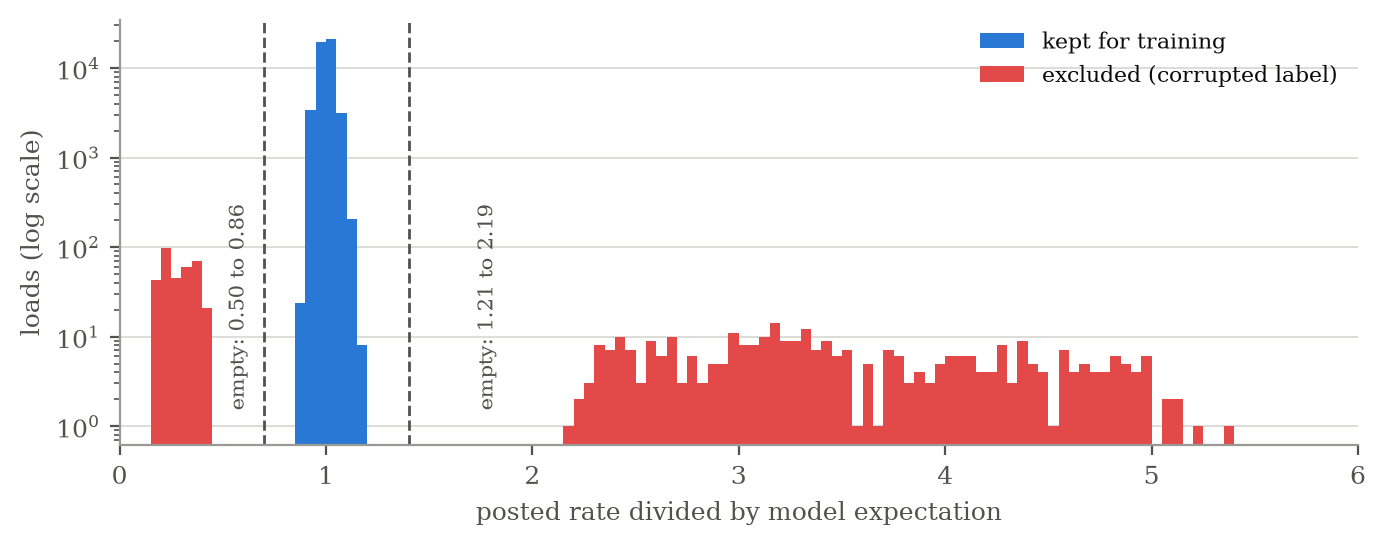
\includegraphics[width=\textwidth]{fig_corruption.png}
\caption{Ratio of posted rate to the model's expectation, on log counts. The
regions on either side of the clean peak are genuinely empty, so the cut points
at 0.70 and 1.40 (dashed) are read directly off the data rather than tuned.}
\end{figure}

Because the two clusters are symmetric, they leave the median almost untouched.
This is therefore noise to be removed rather than a bias to be corrected, and
predictions are deliberately not inflated to chase the corrupted mass. Excluding
these rows is worth more than any modelling decision: leaving them in raises
holdout MAE from \$33 to \$75.

\begin{table}[H]
\small
\begin{tabularx}{\textwidth}{L{0.33\textwidth}R{0.08\textwidth}R{0.08\textwidth}X}
\toprule
\textbf{Issue} & \textbf{Rows} & \textbf{Share} & \textbf{Treatment} \\
\midrule
label corrupted (ratio outside gate) & 677 & 1.41\% & excluded from training \\
weight sign-flipped (negative) & 292 & 0.61\% & absolute value \\
weight missing & 300 & 0.62\% & median impute + flag \\
market\_index missing & 374 & 0.78\% & daily market mean + flag \\
weight at 47,500 cap & 1{,}204 & 2.51\% & flagged (upstream cap) \\
distance at 70-mile floor & 48 & 0.10\% & flagged (short-haul minimum) \\
8 cities present only in the validation file & 1{,}447 & 12.1\% & Coordinates used, never city identity \\
\bottomrule
\end{tabularx}
\end{table}

Two further checks returned clean results and so required no treatment. Billed
distance tracks great-circle distance at a stable road-circuity ratio of 1.18,
which rules out corrupted distances, and every city's coordinates are internally
consistent across both files. The 70-mile floor on distance is a genuine
short-haul billing minimum rather than an error, so it is flagged as a feature
rather than repaired.


\section{Validation approach and data split}

The split has to answer the question the task actually poses: how well does the
model price loads in months it has never seen? A random $K$-fold cannot answer
that, because it allows the model to learn from late-October days while scoring
mid-October ones. Running both protocols on an identical model shows how much
that flatters the result.

\begin{figure}[H]
\centering
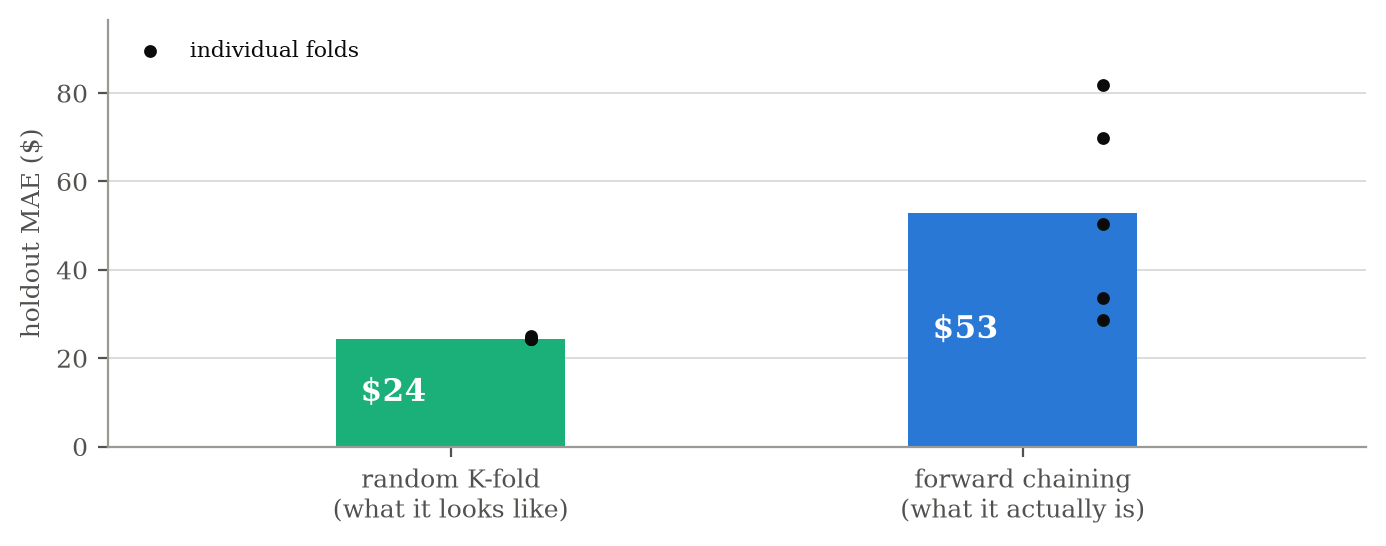
\includegraphics[width=\textwidth]{fig_split.png}
\caption{The same model and the same data under two protocols. Random
$K$-fold reports MAE \$24, while forward chaining
reports \$53. Every modelling decision in this
report was made on the forward-chaining figure.}
\end{figure}

\subsection{Forward chaining}

The training window is expanded one month at a time, and the model is always
scored on the month that follows. This matches the shape of the real task and is
repeated five times.

\begin{table}[H]
\small
\begin{tabularx}{\textwidth}{XlR{0.13\textwidth}R{0.11\textwidth}R{0.11\textwidth}R{0.10\textwidth}R{0.10\textwidth}}
\toprule
\textbf{Train through} & \textbf{Scored on} & \textbf{Train rows} &
\textbf{Holdout} & \textbf{MAE} & \textbf{MAPE} & \textbf{$R^2$} \\
\midrule

End of May & June & 24{,}023 & 4{,}783 & \$69.77 & 2.74\% & 0.9957 \\
End of June & July & 28{,}806 & 4{,}912 & \$50.27 & 2.08\% & 0.9974 \\
End of July & August & 33{,}718 & 4{,}759 & \$81.82 & 3.34\% & 0.9919 \\
End of August & September & 38{,}477 & 4{,}670 & \$33.58 & 1.42\% & 0.9988 \\
End of September & October & 43{,}147 & 4{,}853 & \$28.70 & 1.26\% & 0.9991 \\
\midrule
 & \textbf{Mean} & & & \textbf{\$52.83} &
\textbf{2.17\%} &
\textbf{0.9966} \\
\bottomrule
\end{tabularx}
\end{table}

Error falls steadily as the window grows. The June fold trains on five months and
reaches MAE \$70, while the October fold trains on nine months and reaches \$29.
The final model is therefore fitted on all ten months of development data.

\subsection{A two-month holdout matching the real horizon}

The submission must reach 61 days past the last training row, so the headline
check trains through August and predicts September and October together. This is
the figure quoted in the summary.

\begin{table}[H]
\small
\begin{tabularx}{\textwidth}{XR{0.12\textwidth}R{0.11\textwidth}R{0.11\textwidth}R{0.11\textwidth}R{0.10\textwidth}R{0.10\textwidth}}
\toprule
\textbf{Model} & \textbf{Train} & \textbf{Holdout} & \textbf{MAE} &
\textbf{RMSE} & \textbf{MAPE} & \textbf{$R^2$} \\
\midrule
Hybrid (shipped) & 38{,}477 & 9{,}523 & \$33.16 & \$47.30 & 1.42\% & 0.9988 \\
Linear base only & 38{,}477 & 9{,}523 & \$65.59 & \$91.93 & 2.99\% & 0.9955 \\
\bottomrule
\end{tabularx}
\end{table}

\subsection{Holding out whole cities}

No time-based split can test the 8 cities that appear only in the validation
file, because every city in the development data is present throughout it. A
second protocol therefore holds out 8 entire cities at a time and scores only
the loads that touch them, repeated five times.

\begin{table}[H]
\small
\begin{tabularx}{\textwidth}{XR{0.14\textwidth}R{0.14\textwidth}R{0.16\textwidth}}
\toprule
\textbf{Variant} & \textbf{MAE} & \textbf{MAPE} & \textbf{Mean bias} \\
\midrule
Shipped model (coordinates) & \$28.51 & 1.17\% & +0.05\% \\
Geography removed & \$30.37 & 1.31\% & +0.13\% \\
\bottomrule
\end{tabularx}
\end{table}

On loads involving a city it has never seen, the model still reaches
1.17\% MAPE with +0.05\%
bias, so the 8 unseen validation cities are not a material risk. This test also
overturned a design decision. An explicit nearest-neighbour regional index, built
specifically to serve unseen cities, scored 2.4\% worse than simply allowing the
trees to use raw coordinates, and was removed from the final model.


\section{Model selection and reasoning}

The model is a trimmed log-linear base combined with a LightGBM correction fitted
to its residuals. The division of labour is deliberate. The base carries every
effect that must extrapolate past the end of the training window, namely the
distance elasticity, both market signals, equipment and the time trend. LightGBM
then learns what the linear form leaves behind, namely curvature in distance and
weight and the regional premium held in the coordinates, using features that all
remain inside ranges already observed.

The reason for not using trees alone is structural rather than empirical. A tree
predicts a constant beyond its last split, so it cannot produce an upward trend
in a period it has never seen. Dropping the time term leaves a systematic
$-$3.4\% shortfall two months
out, against $-$0.16\% when it
is retained. A plain LightGBM trained on raw labels reaches MAE
\$87, against \$33
for the model submitted here.

\begin{figure}[H]
\centering
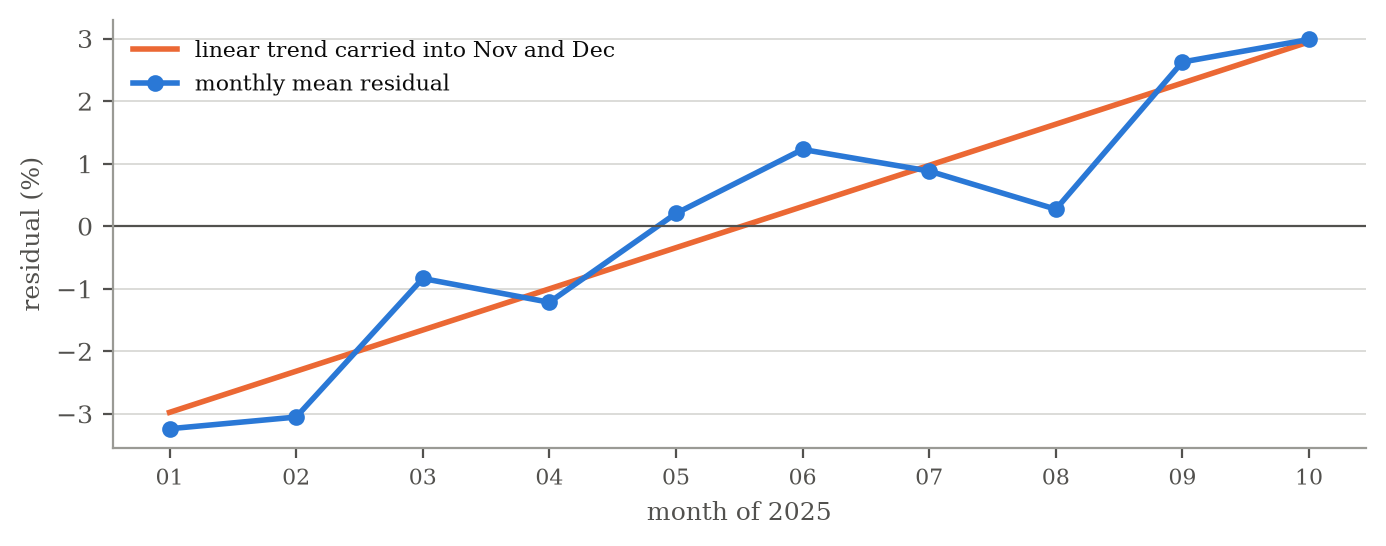
\includegraphics[width=\textwidth]{fig_trend.png}
\caption{Monthly mean residual from a model carrying no time term. The drift is
clear but is not a clean ramp, since it pauses through July and August. A
straight line explains 89\% of the monthly pattern, while quadratic and cubic
terms add almost nothing and are considerably more dangerous 61 days beyond the
last observation. A single linear term is therefore used.}
\end{figure}

\begin{table}[H]
\small
\begin{tabularx}{\textwidth}{XR{0.18\textwidth}R{0.16\textwidth}R{0.16\textwidth}}
\toprule
\textbf{Window fitted} & \textbf{Drift per day} & \textbf{$t$ statistic} &
\textbf{Per 30 days} \\
\midrule
January to March & 0.000415 & 38.2 & +1.25\% \\
April to June & 0.000443 & 41.7 & +1.34\% \\
July and August & $-$0.000145 & $-$7.7 & $-$0.43\% \\
September and October & 0.000322 & 15.6 & +0.97\% \\
Full window, January to October & 0.000218 & 120.6 & +0.66\% \\
\bottomrule
\end{tabularx}
\end{table}

The drift is strongly significant over the full window and positive in three of
the four sub-windows. It is carried forward as a linear term and nothing more
aggressive, which is the conservative reading of a trend that visibly pauses
mid-year.

\subsection{What each decision is worth}

\begin{figure}[H]
\centering
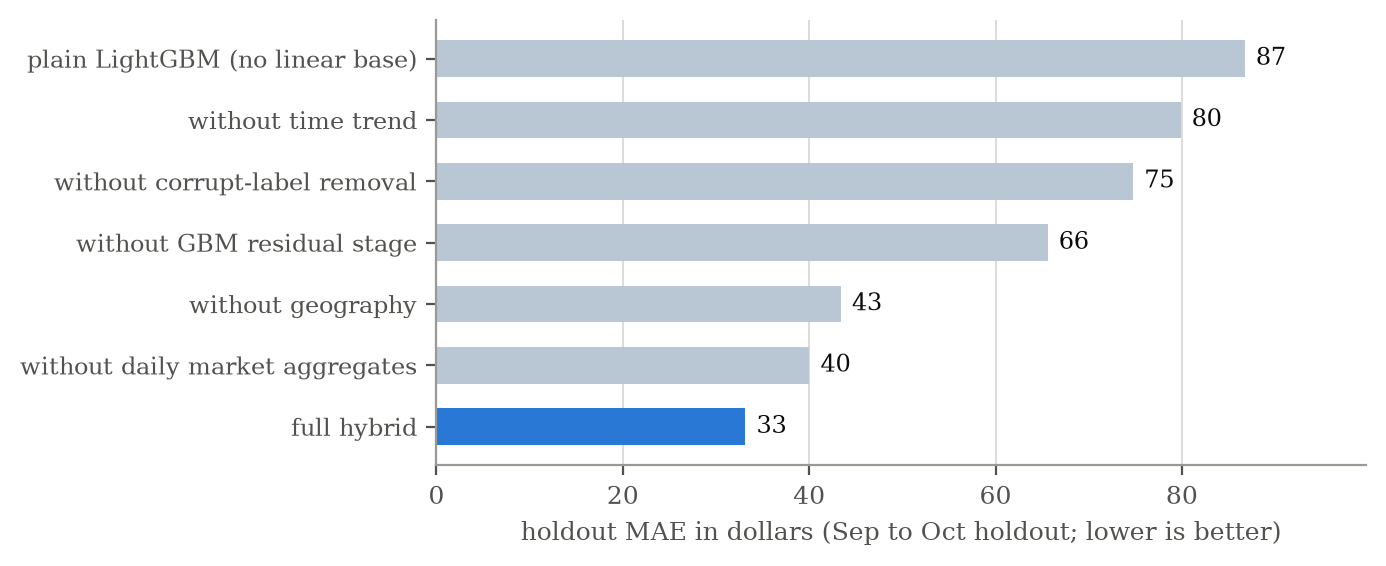
\includegraphics[width=\textwidth]{fig_ablation.png}
\caption{Each variant retrained from scratch and scored on the September and
October holdout. Cleaning the labels and extrapolating the trend matter more
than the choice of learning algorithm.}
\end{figure}

\subsection{Base model coefficients}

\begin{table}[H]
\small
\begin{tabularx}{\textwidth}{L{0.33\textwidth}R{0.16\textwidth}X}
\toprule
\textbf{Term} & \textbf{Coefficient} & \textbf{Interpretation} \\
\midrule

intercept & +0.630387 & Baseline level \\
log\_distance & +0.871203 & 1\% more distance gives 0.87\% more rate \\
log\_weight & +0.080974 & 1\% more weight gives 0.08\% more rate \\
log\_market\_index & +0.129737 & Load-level market reading \\
log\_quote\_signal & +0.008070 & Load-level quote reading \\
log\_market\_index\_daily & +0.033500 & That day's market level \\
log\_quote\_signal\_daily & +0.123083 & That day's quote level \\
days\_elapsed & +0.000225 & 0.0225\% of upward drift per day \\
is\_flatbed & +0.079836 & 8.3\% above Dry Van \\
is\_reefer & +0.121319 & 12.9\% above Dry Van \\
\bottomrule
\end{tabularx}
\end{table}


\newpage
\section{The fixed December chart}

Every input is held constant, namely Lexington to Fort Wayne, 360 miles, Dry Van
and 32{,}000 lb, and only the date varies. The curve therefore isolates what the
model believes about time alone.

\begin{figure}[H]
\centering
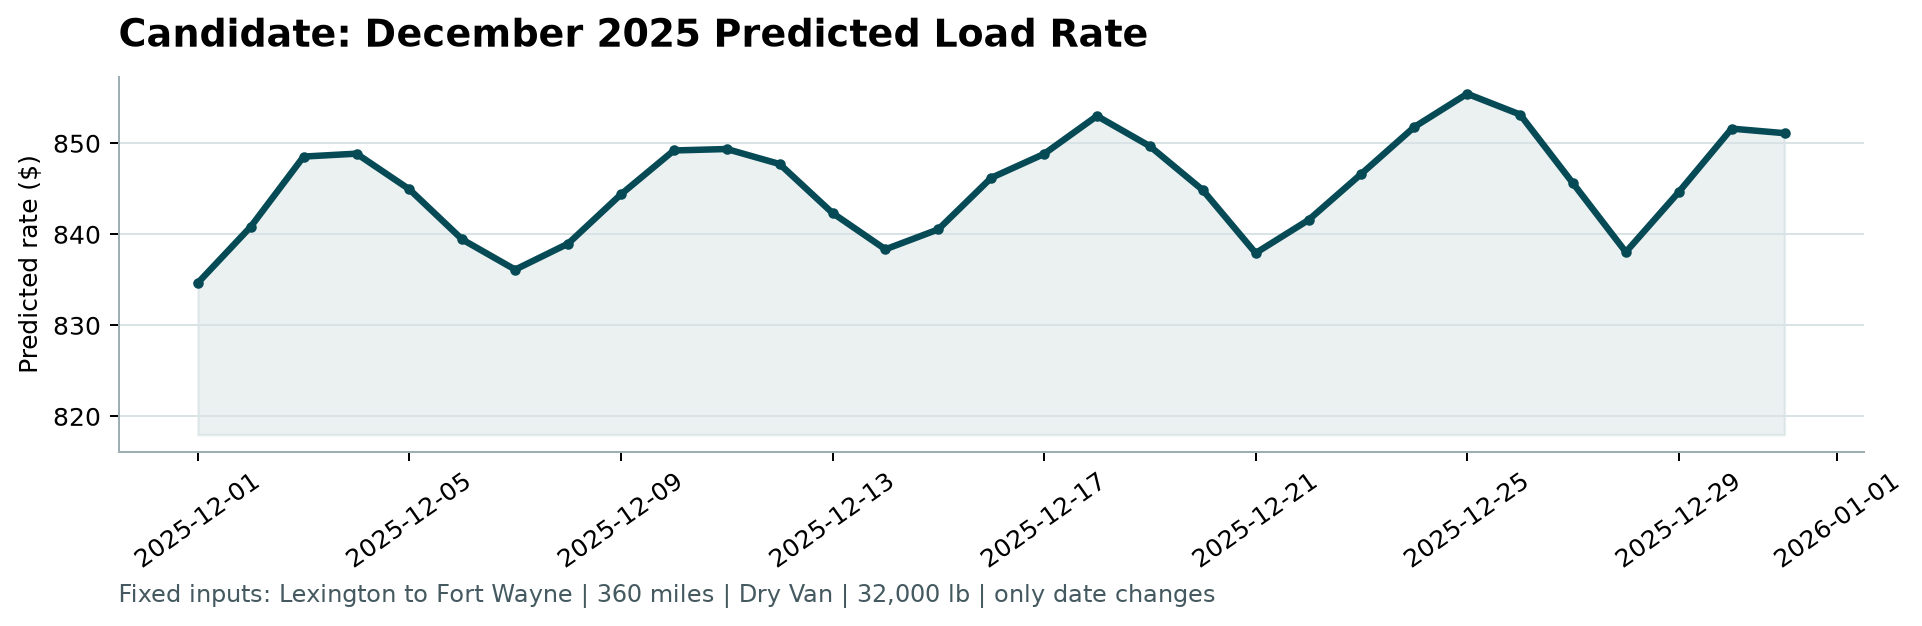
\includegraphics[width=\textwidth]{candidate_december.png}
\caption{Produced by the supplied \texttt{score.py} from the completed
\texttt{data/december\_chart\_inputs.csv}.}
\end{figure}

The chart shows two effects simultaneously. The upward slope across the month is
the time trend carried forward from the development data. The repeating ripple is
the daily market level: the two market columns are published per load, so the
fixed December rows are priced using each day's mean across the 6{,}164 December
loads present in the validation file. That uses no target values, and it is the
only reason these 31 rows can be priced at all. Troughs fall on Sundays and peaks
mid-week, and the range across the whole month is about \$21, or 2.5\%.

The level is independently plausible. Comparable real loads in the development
data, restricted to Dry Van between 300 and 420 miles and 28{,}000 to 36{,}000 lb,
have a median of \$2.35 per mile, which scales to \$846 at 360 miles. The December
predictions average \$845. Actual Lexington to Fort Wayne Dry Van loads in October
posted between \$796 and \$865.


\section{Limitations and next steps}

\begin{table}[H]
\small
\begin{tabularx}{\textwidth}{L{0.27\textwidth}L{0.33\textwidth}X}
\toprule
\textbf{Limitation} & \textbf{Why it is acceptable here} & \textbf{Next step} \\
\midrule
The time trend is extrapolated 61 days on the assumption that it continues & It is positive in three of four sub-windows and strongly significant overall, and a linear term is the conservative choice & Refit weekly as actuals arrive, and alert when realised rates fall outside the residual band \\
Daily market levels for November and December come from the validation file's own feature columns & These are exogenous inputs shipped with every row, labelled or not, so no target value is used & In production the market index is published daily, so this is the same information a live service would hold \\
Approximately 1.4\% of validation labels are likely corrupted as well & Corruption is symmetric and independent of the features, so it inflates the score without biasing it & Report a robust metric alongside MAE so model quality is not confounded with label noise \\
Only 72 cities and 10 months are represented & Geography is handled through coordinates, so new cities interpolate & Retrain as the lane network widens, with attention to the far south-west where neighbours are sparse \\
\bottomrule
\end{tabularx}
\end{table}

\subsection*{Reproducing these results}

All figures in this report are regenerated from the repository by running
\texttt{python -m src.validate}, \texttt{python -m src.ablation},
\texttt{python -m src.unseen\_cities} and \texttt{python -m src.train\_predict},
in that order. Full setup instructions are in the repository README.

\end{document}
